\documentclass[12pt] {article}
\usepackage{times}
\usepackage[margin=1in,bottom=1in,top=1in]{geometry}

\usepackage{hhline}
\usepackage{subfig}
\usepackage{amsmath}
\usepackage{amsfonts}
\usepackage[inline,shortlabels]{enumitem}%enumerate with letters
\usepackage{mathrsfs} 
\usepackage[square,numbers]{natbib}
\usepackage{graphicx}
\bibliographystyle{unsrtnat}
\begin{document}

\title{Assignment Four -  EEC254}
\author{Ahmed H. Mahmoud}
\date{February 13th, 2018}
\maketitle

%============Table========
%\begin{figure}[tbh]
% \centering    
%\begin{tabular}{ |p{4cm}|| p{2cm}|p{2cm}|p{2cm}|p{2cm}|}
% \hline
% & Processor 1 &  Processor 2  & Processor 3 & Processor 4\\ \hhline{|=|=|=|=|=|}
% \hline
% Performance          &$1.08$        &$1.425$       &\textbf{1.52}  &   \\
% \hline
%\end{tabular} 
%\caption{Metric table for the four processors}
%   \label{tab:metric}
%\end{figure} 
%============Figure========
%\begin{figure}[!tbh]
%\centering        
%   \subfloat {\includegraphics[width=0.65\textwidth]{fig2_4.png}}
%   \caption{ }
%   \label{fig:fig}
%\end{figure}

%\begin{enumerate}[(a)]
%\end{enumerate}


\paragraph{Problem 4.21:} 
(a),(b). We consider first the general case in which the center of the ellipsoid is not the origin (b) and then set the center to be zero to solve (a). Since the function is linear, its minimum must be on the boundary of the ellipsoid. Thus, we can convert the inequality to equality. We use change of variable to scale the ellipsoid such that it becomes a unit ball. For that we define $y = A^{\frac{1}{2}}(x-x_{c})$. Thus, $x = A^{\frac{-1}{2}}y +x_{c}$. The problem then becomes 
\[
\begin{array}{cl}
\text{minimize} & c^{T}A^{\frac{-1}{2}}y +c^{T}x_{c}\\
\text{subject to} & y^{T}y \leq 1\\
\end{array} 
\]
which is a minimization of linear function over unit ball for which the solution is 
$$
y^{*} = \frac{-A^{\frac{-1}{2}}c}{||A^{\frac{-1}{2}}c||_{2}} \quad \quad x^{*} = x_{c} - \frac{A^{-1}c}{||A^{\frac{-1}{2}}c ||_{2}} \quad \quad p^{*}= c^{T}x_{c} - \frac{c^{T}A^{-1}c}{||A^{\frac{-1}{2}}c ||_{2}}
$$

Thus, the solution for (a) (by setting the center to zero) is 
$$
x^{*} = - \frac{A^{-1}c}{||A^{\frac{-1}{2}}c ||_{2}} \quad \quad p^{*}= - \frac{c^{T}A^{-1}c}{||A^{\frac{-1}{2}}c ||_{2}}
$$
(c) Here we may distinguish between to different cases; 1) one where the optimal value lies inside in the interior of the ellipsoid and 2) one where the optimal value is one the boundary of the ellipsoid. Figure ~\ref{fig:ell} shows the two different cases (here we shifted the ellipsoid but in reality the function is the one that is shifted).

To simplify things, we will use change of variables we used above to convert the problem to minimizing quadratic function over a unit sphere. Let $y = A^{\frac{1}{2}}x$. Thus $x = A^{\frac{-1}{2}}y $ and the problem becomes 
\[
\begin{array}{cl}
\text{minimize} & y^{T}A^{\frac{-1}{2}} B A^{\frac{-1}{2}}y\\
\text{subject to} & y^{T}y \leq 1\\
\end{array} 
\]
When the optimal is inside the ellipsoid, the gradient must be zero. From that we have $A^{\frac{-1}{2}}BA^{\frac{1}{2}}y=0$ and thus the optimal value is zero (since $A \succ 0$). When the optimal is on the boundary of the ellipsoid, this requires $y^{T}y = 1$. This means that the optimal value is the one that obtains the minimum of $A^{\frac{-1}{2}} B A^{\frac{-1}{2}}$ for $A^{\frac{-1}{2}} B A^{\frac{-1}{2}} \neq 0$.

For the nonconvex extension, we will still seek the gradient to be zero (i.e., the optimal value is inside the ellipsoid) and the solution is similar to the convex case. Otherwise, there could be many solutions for the second case. 

\begin{figure}[!tbh]
\centering
\subfloat [Optimal value inside the ellipsoid ] {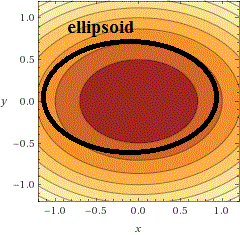
\includegraphics[width=0.45\textwidth]{ell_inside.png}}
\subfloat [Optimal value on the boundary the ellipsoid] {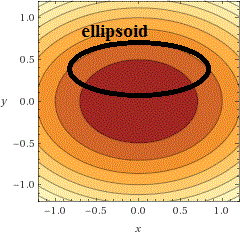
\includegraphics[width=0.45\textwidth]{ell_insect.png}}
   \caption{The two different cases of Problem 4.21 (c). }
   \label{fig:ell}
\end{figure}



\paragraph{Problem 4.40:} 
\begin{enumerate}
\item  \textbf{LP:}
\[
\begin{array}{cl}
\text{minimize} & c^{T}x +d\\
\text{subject to} & diag(Gx - h) \preceq 0\\
&Ax = b
\end{array} 
\]
\item 
\begin{enumerate}
%section 16.8.1 http://users.math.msu.edu/users/markiwen/Teaching/MTH995/Papers/SDP_notes_Marina_Epelman_UM.pdf 
\item \textbf{QP:} The QP is written as 
\[
\begin{array}{cl}
\text{minimize} & x^{T}Px+q^{T}x+r\\
\text{subject to} & Gx \preceq h\\
&Ax = b
\end{array} 
\]
which can be re-written in its epigraph form as 
\[
\begin{array}{cl}
\text{minimize} & t\\
\text{subject to} & x^{T}Px + q^{T}x + r - t \leq 0 \\
& Gx \preceq h\\
&Ax = b
\end{array} 
\]
Since $P$ is symmetric and positive semidefinite, then we can write $P=Q^{T}Q$. From this we have this equivalence  
\[
\left[
\begin{array}{cc}
I & Qx \\
x^{T}Q^{T} & -r-q^{T}x
\end{array} 
\right]
\succeq 0 
\quad \Longleftrightarrow  \quad 
x^{T}Px + q^{T}x + r \preceq 0 
\]
Thus we can write QP as follows 
\[
\begin{array}{cl}
\text{minimize} & t\\

\text{subject to} & \left[ \begin{array}{cc}
                     I & Qx \\
                     x^{T}Q^{T} & -r-q^{T}x + t
                     \end{array} \right] \succeq 0 \\
                   & diag(Gx - h) \preceq 0 \\
&Ax = b
\end{array} 
\]
in $x$ and $t$.
\item \textbf{QCQP:} The QCQP is written as 
\[
\begin{array}{cl}
\text{minimize} & x^{T}P_{0}x+q_{0}^{T}x+r_{0}\\
\text{subject to} & x^{T}P_{i}x+q_{i}^{T}x+r_{i} \leq 0, \quad i=1,\cdots,m\\
&Ax = b
\end{array} 
\]
Following the same logic in QP reformation and apply the equivalence to the constraints as well, we can rewrite QCQP problem as follows 
\[
\begin{array}{cl}
\text{minimize} & t\\

\text{subject to} & \left[ \begin{array}{cc}
                     I & Q_{0}x \\
                     x^{T}Q_{0}^{T} & -r_{0}-q_{0}^{T}x + t
                     \end{array} \right] \succeq 0 \\
                     \\
                  &  \left[ \begin{array}{cc}
                     I & Q_{i}x \\
                     x^{T}Q_{i}^{T} & -r_{i}-q_{i}^{T}x
                     \end{array} \right] \succeq 0, \quad i=1,\cdots, m \\
                  &Ax = b
\end{array} 
\]
in $x$ and $t$.
 
\item \textbf{SOCP:}
The SOCP is written as 
\[
\begin{array}{cl}
\text{minimize} & f^{T}x\\
\text{subject to} & ||A_{i}x +b_{i} ||_{2} \leq c_{i}^{T}x+d_{i}, \quad i=1,\cdots,m\\
&Fx = g
\end{array} 
\]
From the given hint (Schur complement), we can rewrite the constraints in matrix form and the problem becomes 
\[
\begin{array}{cl}
\text{minimize} & f^{T}x\\
\text{subject to} & \left[ \begin{array}{cc}
                     (c_{i}^{T}x+d_{i})I & A_{i}x+b_{i} \\
                     (A_{i}x+b_{i})^{T} & c_{i}^{T}x+d_{i} \\
                     \end{array} \right] \succeq 0 \quad i=1,\cdots,m\\
&Fx = g
\end{array} 
\]
\end{enumerate}
%page 201 https://ac.els-cdn.com/S0024379598100320/1-s2.0-S0024379598100320-main.pdf?_tid=a74d4f58-102d-11e8-8b22-00000aacb360&acdnat=1518465070_34dd186466ba8d450d40f6eabdb40beb
\item We take $F(x) \succ 0 $ as the constraints of the problem. It follows directly from Schur complement that the problem can be re-written as 
\[
\begin{array}{cl}
\text{minimize} & t\\
\text{subject to} & \left[ \begin{array}{cc}
					F(x)       & Ax+b\\
					(Ax+b)^{T} & t
                     \end{array} \right] \succeq 0 \\
\end{array} 
\]




\end{enumerate}
\paragraph{Problem 4.42:} 
In order to prove the relation we shall use the definition of positive semi-definite Hermitian matrix. Let $c$ be a complex vector such that $c= u+iv$. Then we have $c^{H}Xz = (u-iv)^{T}(\mathscr{R}X + i\mathscr{I}X)(u+iv)$. This equation can be written in matrix form as 

\[
\left[
\begin{array}{cc}
u^{T} & v^{T}
\end{array} 
\right]
\left[
\begin{array}{cc}
\mathscr{R}X & -\mathscr{I}X\\
\mathscr{I}X & \mathscr{R}X
\end{array} 
\right]
\left[
\begin{array}{c}
u\\
v
\end{array} 
\right]
\]
The above is only (component-wise) greater than or equal to zero iff $X\succeq 0$. The conversion is done by breaking down the complex LMI into two pieces; one for the real part and the other for the complex part and operate on them separately. 
\paragraph{Problem 4.50:} 
\begin{enumerate}[(a)]
\item From the plot $||x_{ls}||_{2} \approx 2.5$
\item From the plot $||Ax_{ls} - b||_{2} \approx 2.5$
\item We look for the point for the point where $x=0$ and check the corresponding $||Ax-b||^{2}_{2}$ which becomes just $||-b||^{2}_{2}$ . Thus $||b||_2=\sqrt{10}$.
\item The optimal value $\approx 5$
\item The optimal value $\approx 5$
\item The optimal value $\approx 8$
\item Since $A\in \mathbb{R}^{100\times 10}$ and the solution for $||Ax-b||^{2}$ is unique, then $rank(A)=10$.
\end{enumerate}
 
\bibliography{mybib}
\end{document}
